\documentclass[fleqn,10pt]{wlscirep}
\usepackage[utf8]{inputenc}
\usepackage[T1]{fontenc}
\usepackage{caption}
\usepackage{subcaption}
\usepackage{setspace}
\usepackage{multirow}
\usepackage{epstopdf}
\usepackage{blindtext}
\usepackage{import}
\usepackage[percent]{overpic}
\usepackage{tabularx}
\usepackage{tikz}
\usepackage{hyperref}
\usepackage{float}
\usepackage[figurename=SI Figure]{caption}
\usepackage[tablename=SI Table]{caption}

\graphicspath{{./Plots/}}
\title{Downwelling longwave radiation and sensible heat flux observations are critical for surface temperature
and emissivity estimation from flux tower data}

%\addbibresource{My_ref.bib}
\author[1,*]{Gitanjali Thakur}
\author[1,*]{ Stanislaus J. Schymanski}
\author[1]{Kaniska Mallick }
\author[1]{Ivonne Trebs}
\author[1]{Mauro Sulis}
\affil[1]{Luxembourg Institute of Science and Technology, ERIN, Belvaux, L-4422, Luxembourg}

\affil[*]{gitanjali.thakur@list.lu}
\affil[*]{stanislaus.schymanski@list.lu}

\begin{abstract}
Land surface temperature (LST) is a preeminent state variable that controls the energy and water exchange between the Earth’s surface and the atmosphere. At the landscape-scale, LST is derived from thermal infrared radiance measured using space-borne radiometers. In contrast, plot-scale LST estimation at flux tower sites is commonly based on the inversion of upwelling longwave radiation captured by tower-mounted radiometers, whereas the role of the downwelling longwave radiation component is often ignored. We found that ignoring the reflected downwelling longwave radiation leads not only to substantial bias in plot-scale LST estimation, but also have important implications for the estimation of surface emissivity on which LST is co-dependent. The present study proposes a novel method for simultaneous estimation of LST and emissivity at the plot-scale and addresses in detail the consequences of omitting down-welling longwave radiation as frequently done in the literature. Our analysis uses ten eddy covariance sites with different land cover types and found that the LST values obtained using both upwelling and downwelling longwave radiation components are 0.5 to 1.5 K lower than estimates using only upwelling longwave radiation. Furthermore, the proposed method helps identify inconsistencies between plot-scale radiometric and aerodynamic measurements, likely due to footprint mismatch between measurement approaches. We also found that such inconsistencies can be removed by slight corrections to the upwelling longwave component and subsequent energy balance closure, resulting in realistic estimates of surface emissivity and consistent relationships between energy fluxes and surface-air temperature differences. The correspondence between plot-scale LST and landscape-scale LST depends on site-specific characteristics, such as canopy density, sensor locations and viewing angles. Here we also quantify the uncertainty in plot-scale LST estimates due to uncertainty in tower-based measurements using the different methods. The results of this work have significant implications for the combined use of aerodynamic and radiometric measurements to understand the interactions and feedbacks between LST and surface-atmosphere exchange processes.



\end{abstract}
\begin{document}
%
\includepdf[pages=-]{eartharc_dec.pdf}

\flushbottom
\maketitle
% * <john.hammersley@gmail.com> 2015-02-09T12:07:31.197Z:
%
%  Click the title above to edit the author information and abstract
%
\thispagestyle{empty}
\section*{Supplementry Information}

\subsection*{SI1. Abbreviation list}
\begin{table}[H]
\centering
\begin{tabular}{p{2.5cm} p{4.0cm} p{3.0cm}}

%\begin{tabular}{|c|c|} 
\hline

Symbol & Description & Unit\\

\hline
$R_{net}$ & Net radiation & W m$^{-2}$  \\
$H$ & Sensible heat flux & W m$^{-2}$ \\
$LE$ & Latent heat flux & W m$^{-2}$ \\
$G$ & Ground heat flux & W m$^{-2}$ \\
$R_{lem}$ & Emitted longwave radiation & W m$^{-2}$ \\
$\epsilon$ & Surface emissivity & (-)\\
$\sigma$ & Stefan-Boltzmann constant & W m$^{-2}$K$^{-4}$\\
$T_{s}$ & Surface temperature & K\\
$R_{sdwn}$ & Down-welling shortwave & W m$^{-2}$\\
$R_{ldwn}$ & Down-welling longwave & W m$^{-2}$\\
$R_{sref}$ & Reflected shortwave & W m$^{-2}$\\
$\alpha$ & Surface albedo & (-)\\
$m$ & Aerodynamic conductance to heat transport & $(m/s)$\\
$\epsilon$ 31 & Spectral emissivity for wavelength of 11 $\mu$m & (-) \\
$\epsilon$ 32 & Spectral emissivity for wavelength of 12 $\mu$m & (-)  \\
BADAM & Ameriflux dataset & (-) \\
TERRA & NASA scientific research satellite & (-)  \\
NATT & North Australian Tropical Transect & (-) \\
\hline
\end{tabular}
\caption{Abbreviation list}
\label{table:SI2}
\end{table}


\subsection*{SI2. Comparison table of plot-scale LST with landscape LST using landscape and plot-scale $\epsilon$}
\begin{table}[H]
\centering
\begin{tabular}{|c|c|c|c|c|c|c|c|c|c|c|c|}
 \hline
 \multirow{3}{*}{\textbf{Sites}} & \multicolumn{5}{c}{Landscape-scale $\epsilon$} \vline & \multicolumn{6}{c}{Plot-scale $\epsilon$} \vline \\\cline{2-12}
&  \multirow{2}{*} {$\epsilon$} &  \multicolumn{2}{c}{seq} \vline &  \multicolumn{2}{c}{leq} \vline 
&  \multicolumn{3}{c}{seq} \vline &  \multicolumn{3}{c}{leq}\vline\\ \cline{3-12}
& & $R^2$ & bias & $R^2$ & bias & opt $\epsilon$ & $R^2$ & bias & opt $\epsilon$ & $R^2$ & bias  \\
\hline
SP & 0.974 & 0.80 & -3.67 & 0.81 & -4.61 & 0.96 & 0.81 & -3.0 & 0.85 & 0.82 & -1.91\\
\hline 
AS & 0.974 & 0.93 & -4.78  &0.93  & -6.31 & 0.96 & 0.93  & -3.4 & 0.82 & 0.93 & -1.92  \\ 
 \hline 
TT & 0.974 & 0.55 & -6.76 & 0.57 & -8.30 & 0.95 & 0.58  & -5.06 & 0.80 & 0.52 & -4.02 \\
 \hline
HS & 0.985 & 0.16 & -8.89 & 0.16 & -9.90 & 0.92 & 0.21  & -4.78 & 0.6 & 0.22 & -2.47\\
 \hline
LF & 0.985 & 0.40 & -10.0 & 0.41 & -11.0 & 0.92 & 0.40  & -4.41 & 0.6 & 0.41 & -2.57 \\
 \hline
AR & 0.985 & 0.18 & -2.61 & 0.27 & -3.51 & 0.997 & 0.23  & -2.93 & 0.96 & 0.252 & -2.98\\
 \hline
 DU & 0.985 & 0.80 & -3.67 & 0.81 & -4.61 & 0.99 & 0.428  & -3.682 & 0.985 & 0.425 & -3.926\\
 \hline
TUM & 0.983 & 0.82 &-2.27& 0.84 & -2.10 & 0.99 & 0.89  & 0.99 & 0.97 & 0.89 & 1.93\\
 \hline
BR &0.983 &0.937  &0.525 & 0.937 &-0.195  & 0.98 & 0.917 & 1.87 & 0.82 & 0.895 & 2.72\\
 \hline
YA & 0.974 & 0.855 &-2.081 & 0.855 & -3.45 & 0.97& 0.522 &-4.517 & 0.93 & 0.793 & -0.582\\
 \hline
\end{tabular}
 \caption{ Comparison of plot-scale LST with landscape-scale daytime LST (MODIS, MODA001) at TERRA daily time of pass. Plot scale LST is obtained using landscape-scale emissivity (MODIS $\epsilon$) (left column) and plot-scale emissivity obtained considering no intercept in $H$ and $\Delta T$ (Optimum $\epsilon$) at study sites. The reported plot-scale emissivity are median values and landscape emissivity are  using channel 31 and 32 of MODA001 dataset. Bias is defined as mean of $T_{s} - T_{MODIS}$, $R^{2}$ is coefficient of determination between plot-scale LST in comparison to landscape-scale LST. The site acronyms can be found in \textbf{Table 2} of the main paper.} 
\label{table:SI2_optlstandmod}  
\end{table}
\subsection*{SI3. Emissivity estimation at Howard Springs and negative $T_{s}-T_{a}$ }
\begin{figure}[H]
	\begin{subfigure}{\textwidth}
		\begin{overpic}[width=0.45\textwidth]{hS_seq_2018-05} % ,grid,tics=10
			\put (18,56){\textbf{a}}
		\end{overpic}
		\begin{overpic}[width=0.45\textwidth]{hS_le_2018-05} % ,grid,tics=10
			\put (18,56){\textbf{b}}
		\end{overpic}
	\end{subfigure}
	\setlength{\belowcaptionskip}{-3ex}
	\caption{Monthly daytime ($R_{n} > 25 Wm^{-2}$) $H$ and $\Delta T$ regression plots at Howard Springs using short and long equation. The value of optimised emissivity along with the year and month are shown on top of the plot. 
	}
	\label{fig:hs_hdt}
\end{figure}
 
\subsection*{SI4. $T_{s}$ sensitivity to emissivity at Alice spring and Tumbarumba}
\begin{figure}[H]
	\begin{subfigure}{\textwidth}
		\begin{overpic}[width=0.45\textwidth]{Alice_spring_longw.png} % ,grid,tics=10
			\put (16,75){\textbf{a}}
		\end{overpic}
		\begin{overpic}[width=0.45\textwidth]{TUM_longw} % ,grid,tics=10
			\put (16,75){\textbf{b}}
		\end{overpic}
	\end{subfigure}
	\setlength{\belowcaptionskip}{-3ex}
	\caption{Timeseries of up-welling and down-welling longwave at sites having different land cover. (a) Alice Springs a mulga site. (b) Tumbarumba wet eucalypt forest
	}
	\label{fig:longwave}
\end{figure}

\subsection*{SI5. Variation of RMSE for monthly of $H (\Delta T)$ plot with surface emissivity }
 \begin{figure}[H]
	\begin{subfigure}{\textwidth}
		\begin{overpic}[width=0.45\textwidth]{AS_RMSE_2018} % ,grid,tics=10
			\put (14,69){\textbf{a}}
		\end{overpic}
		\begin{overpic}[width=0.45\textwidth]{tum_RMSE_2017} % ,grid,tics=10
			\put (14,71){\textbf{b}}
		\end{overpic}
	\end{subfigure}
	\setlength{\belowcaptionskip}{-3ex}
	\caption{The RMSE and emissivity for $H(\Delta T)$ linear fit using long equation (a) Alice Spring (b) Tumbarumba
	}
	\label{fig:rmse_eps}
\end{figure}


\subsection*{SI6. Sensitivity of short and long equation to surface emissivity}
\begin{figure}[H]
	\begin{subfigure}{\textwidth}
		\begin{overpic}[width=0.45\textwidth]{Alice_spring_Ts_sensitivity_2005} % ,grid,tics=10
			\put (16,64){\textbf{a}}
		\end{overpic}
		\begin{overpic}[width=0.45\textwidth]{Tum_Ts_sensitivity_2016} % ,grid,tics=10
			\put (16,64){\textbf{b}}
		\end{overpic}
	\end{subfigure}
	\setlength{\belowcaptionskip}{-3ex}
	\caption{Sensitivity of LST estimated using two equations to the range of Broadband emissivity The black dots and blue Stars depicts LST using short (\textbf{Eq. 7} of main paper) and long (\textbf{Eq. 12} of main paper). Midday longwave measurement for 15June, 2016 at Alice Springs and Tumbarumba is used}
	\label{fig:LST sensitivity to emissivity}
\end{figure}



\subsection*{SI7. Energy imbalance closure reduces the correction in measured the up-welling longwave at Howard Springs}
\label{Subsection:wnimb}
\begin{figure}[H]
	\begin{subfigure}{\textwidth}
		\begin{overpic}[width=0.45\textwidth]{rlup_br_hs.png} % ,grid,tics=10
			\put (16,57){\textbf{a}}
		\end{overpic}
		\begin{overpic}[width=0.45\textwidth]{hs_lst_cor.png} % ,grid,tics=10
			\put (22,53){\textbf{b}}
		\end{overpic}
	\end{subfigure}
	\setlength{\belowcaptionskip}{-3ex}
	\caption{(a) Sensible heat flux as a function of surface-to-air temperature difference based on \textbf{Eq.10} of the main paper. Same analysis and legends as in \textbf{Fig 4c} of main paper, but after adding 35 ($W m^{-2}$) to measured $R_{lup}$ and closing the energy balance using a Bowen ratio closure scheme. (b) Comparison of surface temperatures from (a) with landscape scale LST from MODIS. 
	}
	\label{fig:Rlup_ebc}
\end{figure}

\subsection*{SI8. SOBOL based uncertainity in epsilon and LST using long equation with accepting intercept in $H(\Delta T)$ and without intercept in $H(\Delta T)$}
\label{Subsection:intercept}
\begin{figure}[H]
	\begin{overpic}[width=0.45\textwidth]{3_blocks_eps_unc} % 
		\put (12,50){\textbf{a}}
	\end{overpic}
	\begin{overpic}[width=0.45\textwidth]{tsta_interc} % ,grid,tics=10
		\put (14,62){\textbf{b}}
	\end{overpic}
	\setlength{\belowcaptionskip}{-3ex}
	\caption{(a) Uncertainty in plot-scale $\epsilon$ using the short equation and long equation (with and without intercept in $H$ and $\Delta T$ plots). (b) Uncertainty in hourly $\Delta T$ using long equation with and without intercept for July 15. 
	}
	\label{fig:unc_intrc}
\end{figure}







\end{document}

\section*{Results}

Up to three levels of \textbf{subheading} are permitted. Subheadings should not be numbered.

\subsection*{Subsection}

Example text under a subsection. Bulleted lists may be used where appropriate, e.g.

\begin{itemize}
\item First item
\item Second item
\end{itemize}

\subsubsection*{Third-level section}
 
Topical subheadings are allowed.

\section*{Discussion}

The Discussion should be succinct and must not contain subheadings.

\section*{Methods}

Topical subheadings are allowed. Authors must ensure that their Methods section includes adequate experimental and characterization data necessary for others in the field to reproduce their work.

\bibliography{sample}

\noindent LaTeX formats citations and references automatically using the bibliography records in your .bib file, which you can edit via the project menu. Use the cite command for an inline citation, e.g.  \cite{Hao:gidmaps:2014}.

For data citations of datasets uploaded to e.g. \emph{figshare}, please use the \verb|howpublished| option in the bib entry to specify the platform and the link, as in the \verb|Hao:gidmaps:2014| example in the sample bibliography file.

\section*{Acknowledgements (not compulsory)}

Acknowledgements should be brief, and should not include thanks to anonymous referees and editors, or effusive comments. Grant or contribution numbers may be acknowledged.

\section*{Author contributions statement}

Must include all authors, identified by initials, for example:
A.A. conceived the experiment(s),  A.A. and B.A. conducted the experiment(s), C.A. and D.A. analysed the results.  All authors reviewed the manuscript. 

\section*{Additional information}

To include, in this order: \textbf{Accession codes} (where applicable); \textbf{Competing interests} (mandatory statement). 

The corresponding author is responsible for submitting a \href{http://www.nature.com/srep/policies/index.html#competing}{competing interests statement} on behalf of all authors of the paper. This statement must be included in the submitted article file.

\begin{figure}[h!]
\centering
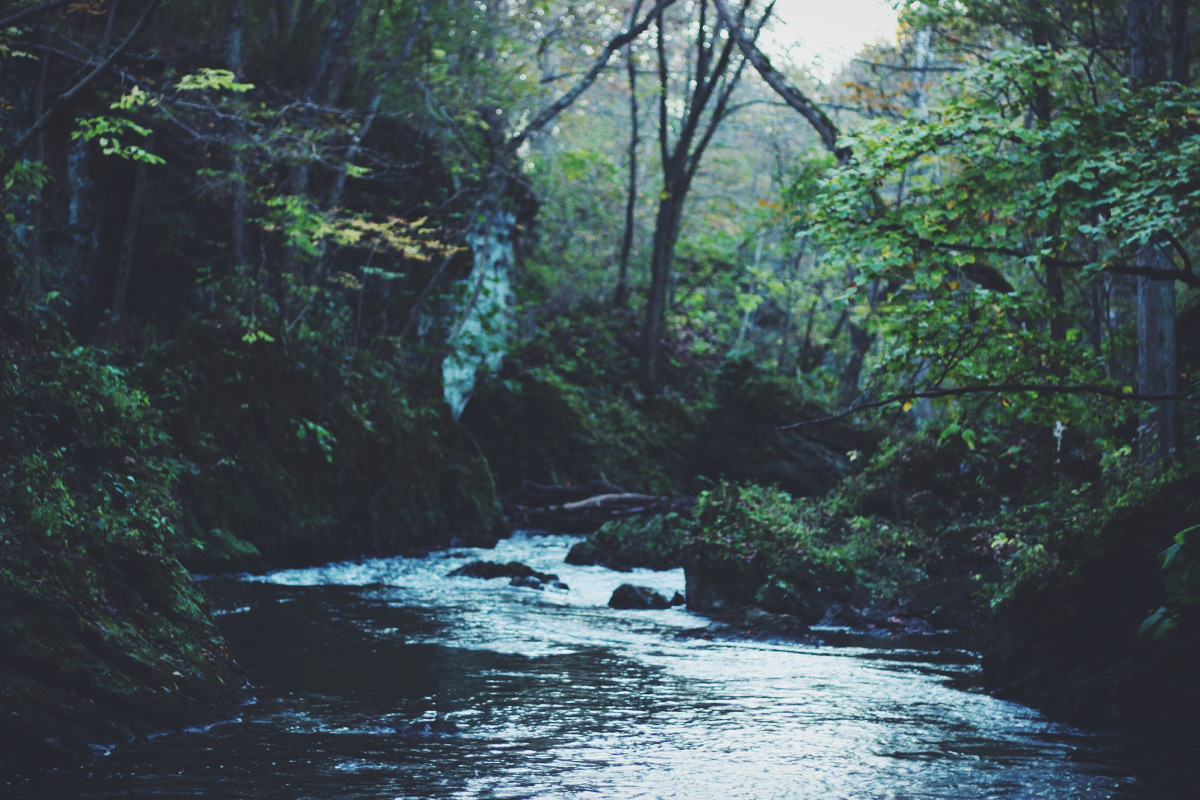
\includegraphics[width=\linewidth]{stream}
\caption{Legend (350 words max). Example legend text.}
\label{fig:stream}
\end{figure}

\begin{table}[ht]
\centering
\begin{tabular}{|l|l|l|}
\hline
Condition & n & p \\
\hline
A & 5 & 0.1 \\
\hline
B & 10 & 0.01 \\
\hline
\end{tabular}
\caption{\label{tab:example}Legend (350 words max). Example legend text.}
\end{table}

Figures and tables can be referenced in LaTeX using the ref command, e.g. Figure \ref{fig:stream} and Table \ref{tab:example}.
\begin{figure}[h!]
\centering
\begin{subfigure}{.5\textwidth}
  \centering
  \includegraphics[width=.95\linewidth]{AS_le_2017-06}
  \caption{H vs Ts -Ta using complete equation for june 2017}
  \label{fig:HDTAsleq}
\end{subfigure}%
\begin{subfigure}{.5\textwidth}
  \centering
  \includegraphics[width=.95\linewidth]{AS_se_2017-06}
  \caption{H vs Ts -Ta using simplified  equation }
  \label{fig:sub2}
\end{subfigure}
\setlength{\belowcaptionskip}{-3ex}
\caption{H vs DT plots using MODIS emissivity}
\label{fig:HDTasseq}
\end{figure}


To include, in this order: \textbf{Accession codes} (where applicable); \textbf{Competing interests} (mandatory statement). 

The corresponding author is responsible for submitting a \href{http://www.nature.com/srep/policies/index.html#competing}{competing interests statement} on behalf of all authors of the paper. This statement must be included in the submitted article file.

\begin{figure}[ht]
\centering
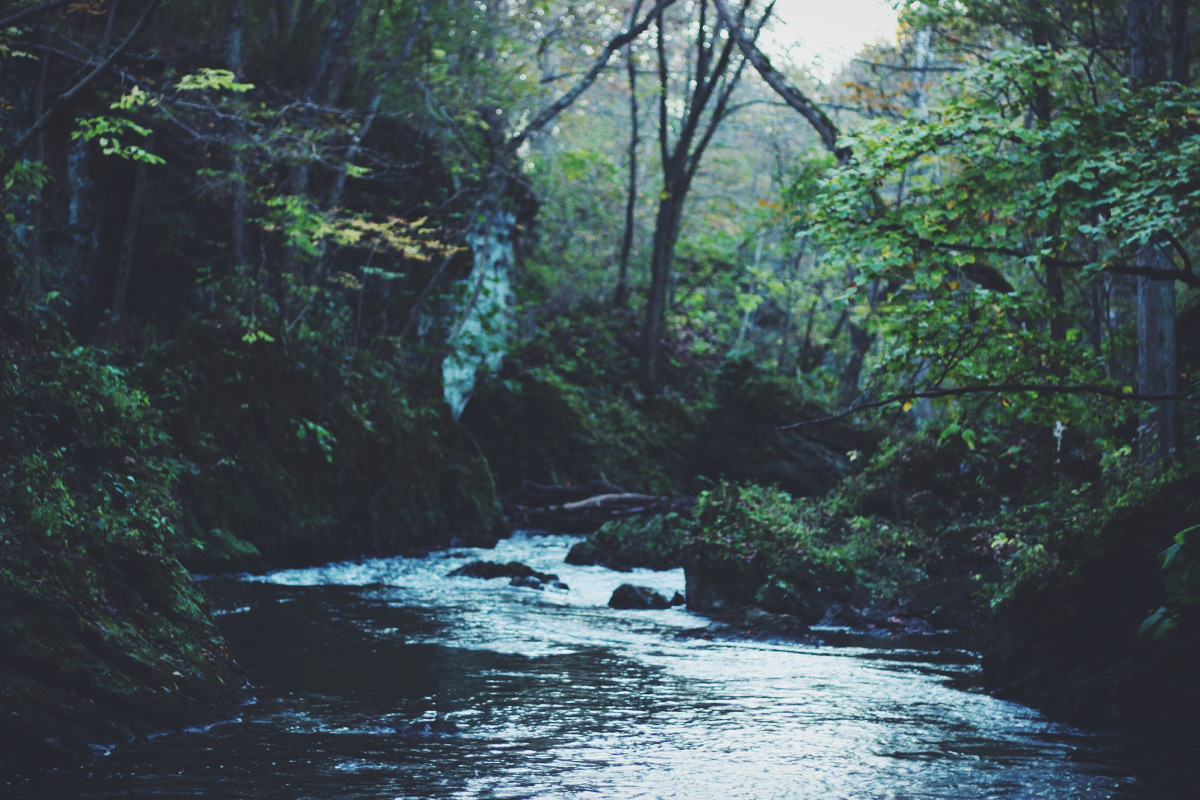
\includegraphics[width=\linewidth]{stream}
\caption{Legend (350 words max). Example legend text.}
\label{fig:stream}
\end{figure}

\begin{table}[ht]
\centering
\begin{tabular}{|l|l|l|}
\hline
Condition & n & p \\
\hline
A & 5 & 0.1 \\
\hline
B & 10 & 0.01 \\
\hline
\end{tabular}
\caption{\label{tab:example}Legend (350 words max). Example legend text.}
\end{table}

Figures and tables can be referenced in LaTeX using the ref command, e.g. Figure \ref{fig:stream} and Table \ref{tab:example}.

\end{document}